\subsection{QuizziPedia::Back-End::Config}
\subsubsection{Informazioni generali}
\label{QuizziPedia::Back-End::Config}
\begin{figure}[ht]
	\centering
	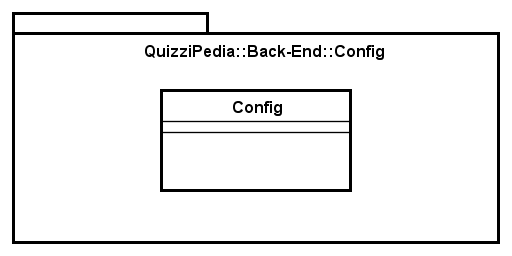
\includegraphics[scale=0.8]{UML/Package/QuizziPedia_Back-End_Config.png}
	\caption{QuizziPedia::Back-End::Config}
\end{figure}
\FloatBarrier
	\begin{itemize}
		\item \textbf{Descrizione}:
		\textit{package\ped{G}} contenente le componenti di configurazione del \textit{server\ped{G}};
		\item \textbf{Padre}: \texttt{Back-End};
		\item \textbf{Interazioni con altri componenti}:
			\begin{itemize}
				\item \texttt{App}:
				\textit{package\ped{G}} contenente le componenti del \textit{server\ped{G}} che implementano il \textit{pattern MVC\ped{G}}.
			\end{itemize}
	\end{itemize}
\subsubsection{Classi}
\paragraph{QuizziPedia::Back-End::Config::Config}
\label{QuizziPedia::Back-End::Config::Config}
\begin{figure}[ht]
	\centering
	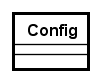
\includegraphics[scale=0.8]{UML/Classi/Back-End/QuizziPedia_Back-End_Config_Config.png}
	\caption{QuizziPedia::Back-End::Config::Config}
	\end{figure}
\FloatBarrier
	\begin{itemize}
		\item \textbf{Descrizione}:
		questa classe gestisce la configurazione del \textit{server\ped{G}}. \textit{Non sono stati modellati attributi e metodi di questa classe in quanto viene gestita da Express\ped{G}};
		\item \textbf{Utilizzo}:
		viene utilizzata per descrivere i parametri dell'applicazione. La classe \texttt{Server} utilizza oggetti di questo tipo per creare ed avviare l'istanza del \textit{server\ped{G}};
		\item \textbf{Relazioni con le altre classi}:
		 \begin{itemize}
		 	\item \textbf{IN} \texttt{Server}:
		 	classe che avvia il \textit{server\ped{G}}. Nello specifico apre una connessione al database tramite \textit{Mongoose\ped{G}}, invoca il \textit{middleware\ped{G}} \textit{Express\ped{G}} passando un riferimento al database \textit{MongoDB\ped{G}} come parametro in modo  che possa configurarsi con esso, invoca il \textit{middleware\ped{G}} \textit{Passport\ped{G}} ed infine si mette in ascolto su una determinata porta. E' il componente \textit{client\ped{G}} del \textit{design pattern\ped{G}} \textit{Chain of responsibility\ped{G}}. Utilizza i moduli \textit{Mongoose\ped{G}}, \textit{Express\ped{G}}, \textit{Passport\ped{G}}.
		 \end{itemize}
	\end{itemize}
